% A distributed maturation delay in the profit-investment cycle
% Self-contained A0 portrait poster (beamerposter). Compile on Overleaf.
% Reuses the figures already in paper/figures/.
\documentclass[final]{beamer}
\usepackage[size=a0,orientation=portrait,scale=1.22]{beamerposter}
\usepackage{graphicx}
\usepackage{amsmath}
\usepackage{booktabs}
\graphicspath{{figures/}}

% --- simple, readable colours ---
\definecolor{accent}{RGB}{18,72,120}
\setbeamercolor{block title}{fg=white,bg=accent}
\setbeamercolor{block body}{fg=black,bg=accent!6}
\setbeamertemplate{navigation symbols}{}
\setbeamertemplate{caption}{\small\insertcaption}
\setbeamerfont{block title}{size=\large,series=\bfseries}

\newlength{\colw}
\setlength{\colw}{0.46\paperwidth}

\begin{document}
\begin{frame}[t]{}

% ===================== HEADER =====================
\begin{beamercolorbox}[wd=\paperwidth,sep=22pt,center]{block title}
  {\veryHuge\bfseries A distributed maturation delay in the\\[10pt]
   profit--investment cycle}\\[18pt]
  {\Large differentiable inverse calibration and identifiability limits}\\[22pt]
  {\large\bfseries Juan I. Tollo \quad\textbar\quad
   Datos, Ecuaciones Diferenciales e Inteligencia Artificial \quad\textbar\quad 2026}
\end{beamercolorbox}
\vspace{1.2cm}

\begin{columns}[t]

% ===================== LEFT COLUMN =====================
\begin{column}{\colw}

\begin{block}{The question}
  \large
  In the overaccumulation tradition (Marx; Goodwin 1967; Tapia Granados 2023),
  \textbf{capital accumulation eventually depresses the rate of profit}, generating
  endogenous business cycles. The classic models (Goodwin's Lotka--Volterra
  predator--prey) impose an \textbf{instantaneous} antagonism with a fixed
  $90^\circ$ phase lag.
  \medskip

  \textbf{We ask:} is the feedback from investment to profits \emph{instantaneous},
  or a \emph{delayed} one whose timing reflects the \textbf{maturation (gestation) of
  investment}? \textbf{We find the latter} --- and then map exactly how far the data
  let us push that claim.
\end{block}

\begin{block}{Data \& methods}
  \large
  Quarterly U.S. corporate profits and gross private investment
  (FRED, 1948--2026, $n=313$), in quarter-over-quarter growth $\Delta\log$
  (the year-over-year transform injects spurious order-4 structure at the lag of
  interest).
  \medskip

  \textbf{Descriptive:} cross-correlation function (CCF) + superposed-epoch event
  study over the 12 NBER recessions.
  \medskip

  \textbf{Physical model.} Investment matures through $n$ stages before depressing
  profits; the linear-chain trick gives a Gamma-distributed delay of mean $\mu$
  (the \emph{maturation lag}):
  \begin{equation*}
    \dot P = c\,I - d\,P - k\,m,\qquad
    \dot I = a\,P - b\,I,\qquad
    m(t)=\textstyle\sum_j w_j(\mu)\,I(t-j).
  \end{equation*}

  \textbf{Differentiable inverse.} We calibrate $(a,b,c,d,k,\mu)$ with an inverse
  physics-informed neural network (PINN): a network $t\mapsto[P,I]$ trained with a
  data loss plus an ODE-residual loss. On long windows a plain network suffers
  spectral bias and the lag collapses; \textbf{Fourier-feature inputs remove this}.
\end{block}

\begin{block}{The pattern: a delayed feedback, not an instantaneous antagonism}
  \large
  The CCF \textbf{oscillates} rather than decaying: a dominant contemporaneous peak
  ($\rho(0)\!\approx\!+0.6$) and a negative lobe at lags 4--5 quarters
  ($\approx\!-0.3$), back to zero by lag~6. The effective phase is near co-movement
  ($\sim\!10^\circ$), \textbf{not} the $90^\circ$ of fixed-phase oscillators --- whose
  CCF is a rigid cosine, so they are refuted.
  \begin{figure}
    \centering
    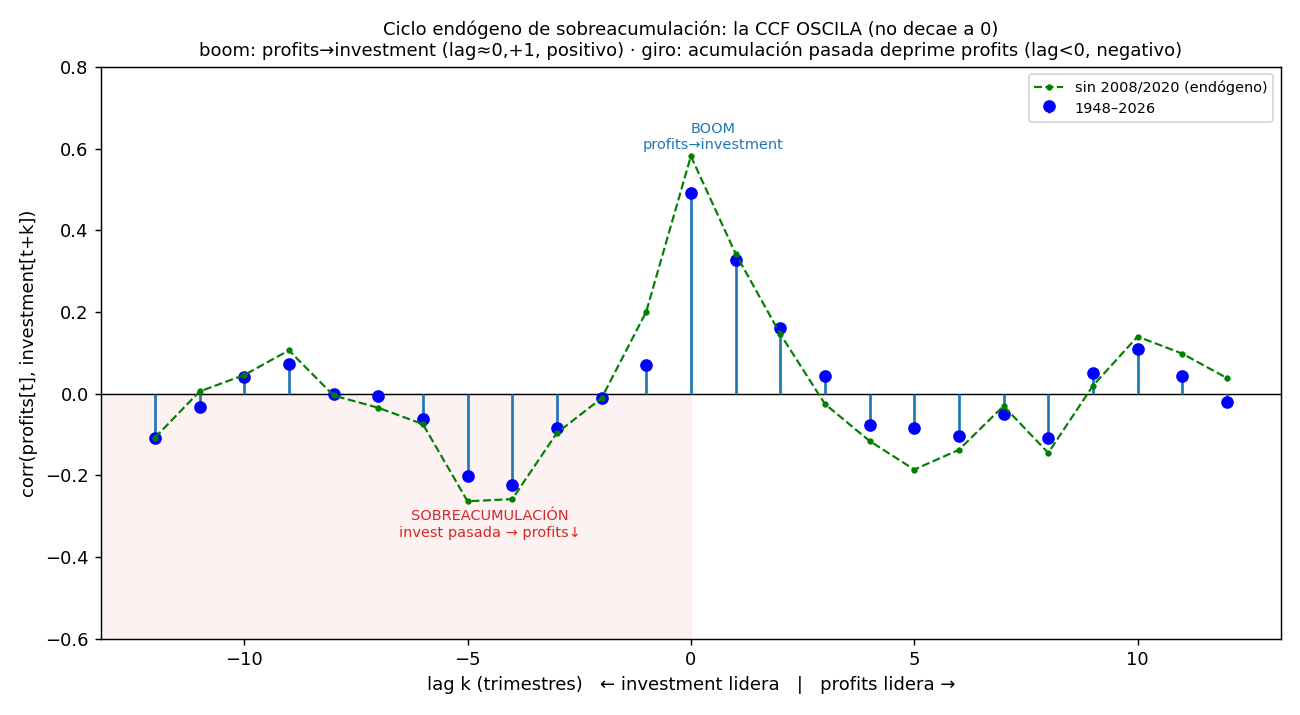
\includegraphics[width=0.92\linewidth]{p7_overaccumulation.png}
    \caption{CCF profits$\leftrightarrow$investment: contemporaneous co-movement
    plus a delayed negative feedback (investment maturing $\sim$1 year earlier
    depresses current profits). Robust to excluding 2008/2020.}
  \end{figure}
  The event study shows profits turning down first and an investment--profit gap that
  \textbf{builds up $\sim$1--1.5 years before the trough} --- the overaccumulation
  buildup of Tapia Granados (2012), re-confirmed by an independent method.
  \begin{figure}
    \centering
    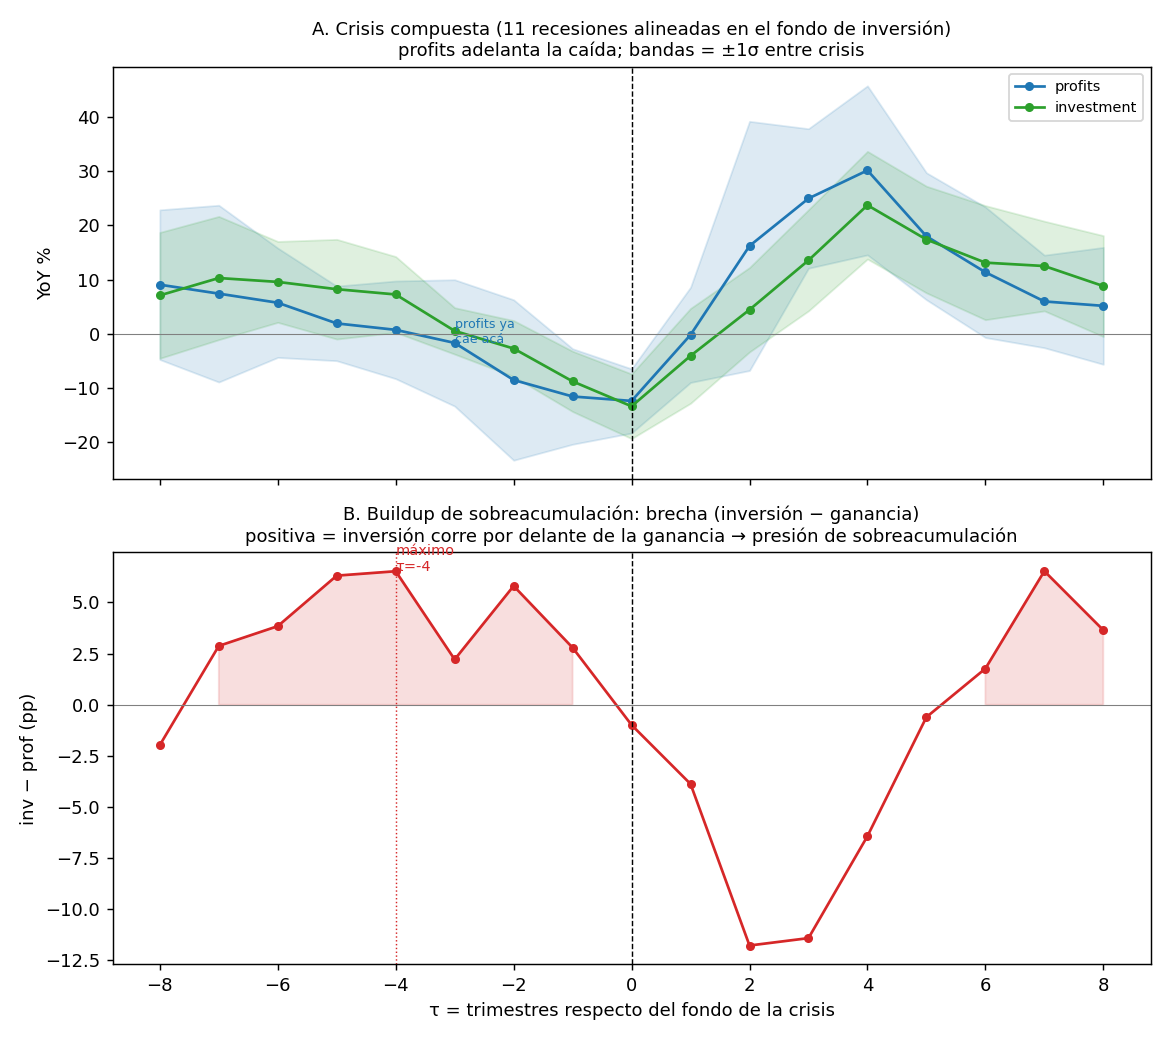
\includegraphics[width=0.92\linewidth]{p8_composite_crisis.png}
    \caption{Composite of NBER recessions aligned at the investment trough.}
  \end{figure}
\end{block}

\end{column}

% ===================== RIGHT COLUMN =====================
\begin{column}{\colw}

\begin{block}{The maturation lag is recovered --- and stable}
  \large
  Five methods converge on a maturation lag of $\approx\!4$ quarters (empirical kernel,
  distributed-lag regression, $\mathrm{VAR}(p\!\ge\!4)$, hierarchical pooling, and the
  differentiable inverse). The \textbf{Fourier-feature inverse PINN} recovers a known
  synthetic lag with $8.9\%$ error and estimates $\mathbf{0.98}$\textbf{ years} on real
  data; the lag is stable to the difference transform and to leave-one-crisis-out.
  \begin{table}\centering\large
    \begin{tabular}{@{}lll@{}}
      \toprule
      Inverse variant & Synthetic (true 4q) & Real lag \\
      \midrule
      Single-shooting / convolution & 1.86q (54\% err) & collapses, non-physical \\
      Per-crisis pooled & 1.64q (59\% err) & 0.84q ($\bar R^2{=}0.86$) \\
      \textbf{Fourier features} & \textbf{4.36q (8.9\%)} & \textbf{0.98 yr} ($R^2{=}1$) \\
      \bottomrule
    \end{tabular}
    \caption{Only Fourier features both fit the series and recover the lag.}
  \end{table}
\end{block}

\begin{block}{Central result: what \emph{cannot} be identified}
  \large
  The feedback explains only $\sim\!3\%$ of the variance of profit growth (vs.\
  $\sim\!35\%$ for the contemporaneous co-movement). Three honest limits follow:
  \medskip

  \begin{itemize}\large
    \item \textbf{Width is not identifiable.} The likelihood profile in the delay
      spread is flat; the data cannot separate a genuinely \emph{distributed}
      (stochastic) delay from a \emph{point} delay.
    \item \textbf{Not crisis-specific.} A kernel placebo over non-crisis windows finds
      the negative lobe roughly as often off-crisis ($p\!=\!0.34$) --- the mechanism is
      \emph{structural and permanent}, not a signature of the turn of the cycle.
    \item \textbf{Observationally equivalent to a linear VAR.} A fitted
      $\mathrm{VAR}(p\!\ge\!4)$ reproduces the negative lobe from its coefficients alone
      (Lyapunov CCF). The maturation model is an interpretable reparameterisation of
      that linear content, not a mechanism separable from it with these data.
  \end{itemize}
  \begin{figure}
    \centering
    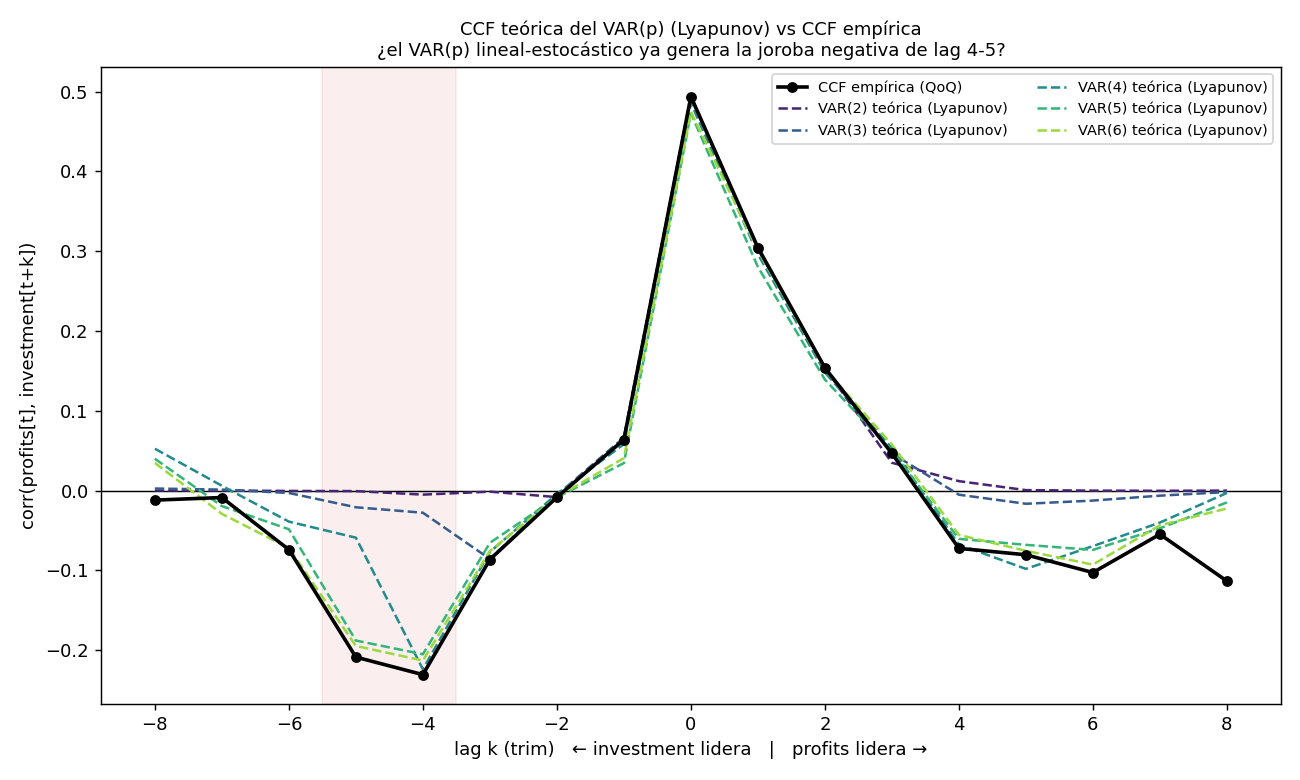
\includegraphics[width=0.86\linewidth]{p12_var_lyapunov_ccf.png}
    \caption{Theoretical CCF of a fitted $\mathrm{VAR}(p)$ vs.\ the empirical CCF: for
    $p\!\ge\!4$ the linear model already reproduces the lag 4--5 lobe.}
  \end{figure}
  A bifurcation analysis finds \textbf{no} delay-induced Hopf instability, so we do
  \emph{not} claim crises to be an endogenous delayed-feedback instability.
\end{block}

\begin{block}{Conclusion}
  \large
  The profit--investment overaccumulation feedback is well described by a
  \textbf{distributed maturation delay centred at $\sim$1 year}, recovered by a
  differentiable inverse that overcomes the spectral bias and ill-posedness of
  classical calibration.
  \medskip

  The robust, transferable result is the \textbf{location of the identifiability
  frontier}: the delay's \emph{centre} is recoverable and stable, while its
  \emph{width} and its \emph{separation from a linear model} are not --- a boundary set
  by signal strength and episode count, not by tuning. \textbf{Pushing past it requires
  new data} (a multi-country panel, or measured sectoral gestation times), not a
  reparameterisation.
\end{block}

\begin{block}{References \& notes}
  \normalsize
  Goodwin (1967); Tapia Granados (2012, 2023); Goldstein (1999); Kalecki (1935);
  Kydland \& Prescott (1982); Raissi et al.\ (2019); Rackauckas et al.\ (2020). \\[4pt]
  \textbf{Data \& code:} FRED public series; full pipeline reproducible (Python + Julia).
  AI tools were used to assist drafting and code; all results verified by the author.
\end{block}

\end{column}
\end{columns}
\end{frame}
\end{document}
